\documentclass[D:/Latex/Internship/Report/Latex/Report.tex]{subfiles}
\usepackage[utf8]{inputenc}
\PassOptionsToPackage{english, british}{babel}
\usepackage[english, british]{babel}
\usepackage{graphicx}
\usepackage{setspace}		%use \doublespacing
\usepackage{hyperref}
\graphicspath{{Figure/}}
\newcommand\NoIndent[1]{%
  \par\vbox{\parbox[t]{\linewidth}{#1}}%
}
\begin{document}
	\chapter{System Design}
	\label{chap:System Design}
		\section{System behavior}
		\label{sec:HardArch}

		\begin{figure}[!ht]
			\label{fig:SystemBlock}
			\centering
			\includegraphics[scale = 0.7]{ControlFlow.pdf}
			\caption{\it System block diagram}
		\end{figure}

		\begin{itemize}
			\item Control flow: The OV7670 Camera module uses an SCCB interface to Control and uses an 8-bits parallel bus to transfer image data. The SCCB interface is similar I2C{\footnote{Inter-Intergrated Circuit}} interface, so we can use the I2C module which has built-in MCU{\footnote{Micro-Controller Unit}} to control the camera. To choose the color format (RGB565 or YCbCr) using Computer through a UART connection.
			\item Dataflow: The Data from the Camera module transfer to DCMI {\footnote{Digital Camera Interface}} module through 8-bits parallel bus. The FIFO of DCMI can store 4 bytes of data, then the data move to SRAM buffer using ${\mu}$DMA{\footnote {Direct Memory Access}}. The data in the buffer will be compressed to jpeg format and send to the Computer using a UART connection.
			\begin{figure}[ht!]
				\centering
				\includegraphics[scale = 0.8]{Figure/DataFlow.pdf}
				\caption{\it Dataflow Structure}
				\label{fig:DataFlow}
			\end{figure}
			\newpage
			\item Timing requirements: System timing is constrained by the frame rate. The OV7670 Camera support 30fps, but Cortex M4 is too slow to process this big data flow. Because the time to receive the data from the camera and the time to transmit UART is too fast compared to the time compress jpeg. Therefore, The time to process jpeg is the time per frame.
			\begin{itemize}
				\item Time per frame = {\Large $ \frac{1}{30} s$}
				\item Jpeg process time per frame:
				\begin{itemize}
					\item 160x120: $t \simeq 160ms$ $\Rightarrow$ $fps \simeq 6fps$
				\end{itemize}
			\end{itemize}

			\item State diagrams:
			\begin{figure}[!ht]
			\label{fig:SystemState}
			\centering
			\includegraphics[scale = 0.7]{StateDiagram.pdf}
			\caption{\it System state diagrams}
			\end{figure}	

			\begin{itemize}
				\item Idle state: This state will start when reset system or after set DMA for the output buffer. 
				\item Start capture state: When the VSYNC{\footnote{Vertical Synchronous}} signal is detected, The CPU {\footnote{Central Processing Unit}} will allow the DCMI module to capture the frame.
				\item Process Line by Line state: To reduce the time process, The image must be process line by line. The time for capture one is smaller than the time for process one line. Therefore, we just using the simple synchronous signal.
				\item Transmit data state: Because the jpeg compression has a different size, depending on the complexity of the photo. The jpeg data must be sent when the compression is done. 						
			\end{itemize}							
		\end{itemize}
	\section{Hardware description}
		\label{sec:Hardware description}
		\subsection{Board Nucleo STM32}
		\label{subsec:Board Nucleo STM32}
			\begin{figure}[h!]
				\centering
				\includegraphics[width = 0.9\linewidth]{Figure/Board.pdf}
				\caption{\it Board NUCLEO STM32F4 F466RE}
			\end{figure}
			\begin{itemize}
				\item Specifications:
				\begin{itemize}
					\item STM32 microcontroller with LQFP64 package.
					\item Two types of extension resources
					\begin{itemize}
						\item Arduino Uno Revision 3 connectivity
						\item STMicroelectronics Morpho extension pin headers for full access to all STM32 I/Os
					\end{itemize}
					\item On-board ST-LINK/V2-1 debugger/programmer with SWD connector
					\begin{itemize}
						\item selection-mode switch to use the kit as a standalone ST-LINK/V2-1
					\end{itemize}
					\item Flexible board power supply
					\begin{itemize}
						\item USB VBUS or external source (3.3V, 5V, 7-12V)
						\item Power management access point
					\end{itemize}
					\item Three LEDs
					\begin{itemize}
						\item USB communication (LD1), user LED (LD2), power LED (LD3)
					\end{itemize}
					\item Two push buttons: USER and RESET
					\item USB re-enumeration capability: three different interfaces supported on USB
					\begin{itemize}
						\item Virtual Com port
						\item Mass storage
						\item Debug port
					\end{itemize}
					\item Supported by wide choice of Integrated Development Environments (IDEs) including $IAR^{TM}$, $Keil^{\circledR}$, GCC-based IDEs
				\end{itemize}
			\end{itemize}
		\subsection{Camera OV7670}
			\begin{figure}[!ht]
				\centering
				\includegraphics[width = 0.6\linewidth]{Figure/OV7670.pdf}
				\caption{\it Camera OV7670 without FIFO}
			\end{figure}
			\begin{itemize}
				\item Specifications:
				\begin{itemize}
					\item Photosensitive Array: 640x480
					\item IO Voltage: 2.5V to 3.0V
					\item Operating Power: 60mW/15fps
					\item Sleeping Mode: <20$\mu$A
					\item Operating Temperature: -30 to 70 deg C
					\item Output Format: YUV/YCbCr4:2:2 RGB565/555/444 GRB4:2:2 Raw RGB Data (8 bits)
					\item Lens Size: 1/6"
					\item Vision Angle: 25 degree
					\item Max Frame Rate: 30fps VGA
					\item Sensitivity: 1.3V / (lux-sec)
					\item Signal to Noise Ratio: 46dB
					\item DynamicRange: 52dB
					\item Browse Mode: By row
					\item Electronic Exposure: 1 to 510 row
					\item Pixel Coverage: 3.6$\mu$m x 3.6$\mu$m
					\item Dark Current: 12mV/s at 60 deg C
					\item PCB Size (L x W): Approx. 1.4x1.4inch / 3.5x3.5cm
				\end{itemize}
			\end{itemize}
		\subsection{Uart to MicroUSB CP2102}
			\begin{figure}[!ht]
				\centering
				\includegraphics[width = 0.5\linewidth]{Figure/CP2102.pdf}
				\caption{\it UART to MicroUSB CP2102}
			\end{figure}
			\begin{itemize}
				\item Features:
					\begin{itemize}
						\item Embedded USB transceiver, no external circuit device
						\item Containing clock circuit, no external circuit device
						\item Contains power-on reset circuit
						\item The on-chip voltage regulator within the 3.3V output
						\item Meet the USB2.0 specification requirements
						\item SUSPEND pins support USB suspend state
						\item Asynchronous serial data bus compatible with all handshakes and modulation controller interface signals
						\item Support data format is 8 data bits, 1 stop bit and the parity bit
						\item Connotation 512 byte receive buffer and 512 byte transmit buffer
						\item Supports hardware or X-ON / X-OFF Handshake
						\item Size: 21x16mm
					\end{itemize}
			\end{itemize}


		\section{Design Hardware}
			\subsection{OV7670 block and connection}
			\begin{figure}[ht!]
			\includegraphics[scale = 0.7]{Figure/OV7670_Functional.pdf}
			\caption{\it Functional block diagram}
			\end{figure}
			\begin{itemize}
				\item Control I/F 
				\begin{itemize}
					\item SCCB (SIO\_C, SIO\_D)
				\end{itemize}
				\item Clock supply
				\begin{itemize}
					\item Supply around 10 to 48MHz
				\end{itemize}
				\item Synchronization
				\begin{itemize}
					\item OV7670 outputs PCLK, HREF and VSYNC
				\end{itemize}
				\item Output data length
				\begin{itemize}
					\item OV7670 outputs 8bit data D[7:0]
				\end{itemize}
			\end{itemize}
			\subsection{Hardware connection}
			\begin{figure}[ht!]
			\centering
			\includegraphics[width = 0.8\linewidth]{Figure/Hardware_connection.pdf}
			\caption{\it Hardware connection}
			\end{figure}			
			\subsection{MCU pinout} 
				\begin{figure}[ht!]
					\centering
					\includegraphics[width = 0.8\linewidth]{Figure/MCU_pinout.pdf}
					\caption{\it MCU pinout}
				\end{figure}
				\newpage
			\subsection{System Architecture}
				\begin{figure}[ht!]
					\centering
					\includegraphics[width = 0.8\linewidth]{Figure/System_Architecture.pdf}
					\caption{\it System Architecture}
				\end{figure}
			\subsection{Schematic}
				\begin{figure}[ht!]
					\centering
					\includegraphics[width = 1\linewidth]{Figure/Schematic.pdf}
					\caption{\it Schematic}
				\end{figure}

	\section{The clock configuration}
	\label{sec:The Clock Configuration}
		\subsection{Main clock tree}
		\label{subsec:Main clock tree}
			Many systems need high performance, the clock configuration is important. To reduce the time's processing is smallest, the core clock of stm32f446re is setup to maximum (180Mhz). The CubeMX tool makes clock setup easier. Figure \ref{fig:Main clock tree} below shows the clock tree of this project. \\
			\begin{figure}[ht!]
				\centering
				\includegraphics[scale = 0.3]{Figure/MainClockTree.png}
				\caption{\it Main clock tree of the CPU}
				\label{fig:Main clock tree}
			\end{figure}

		\subsection{The clock source for the camera module}
		\label{subsec:The clock source for the camera module}
		The OV7670 camera does not contain the crystal clock. If using an external crystal is complex, so using a built-in MCO is a good choice. The camera's clock source has ranged from 10 to 48 Mhz. The MCO of Cotex M4 support from 1 - 5 divider. Therefore, the PLL clock (180Mhz) is divided to 5 and getting 36Mhz (in of range). Clock selection is shown in figure \ref{fig:Clock source for camera} below.\\
			\begin{figure}[ht!]
				\centering
				\includegraphics[scale = 0.5]{Figure/MCO.png}
				\caption{\it Clock source for camera module using MCO}
				\label{fig:Clock source for camera}
			\end{figure}
	\section{Software}
	\label{sec:Software}
		\subsection{Interface}
		\label{sebsec:Interface}
		\begin{enumerate}
			\item Serial camera control bus (SCCB)
			\begin{figure}[ht!]
			
				\centering
				\includegraphics[scale = 1.2]{ov_SCCB_Connect.pdf}
				\caption{\it Serial camera control bus connection}
				\label{fig:sccbConnect}
			\end{figure}

			\noindent{The Serial Camera Control Bus interface controls the Camera Chip sensor operating. The SCCB interface is similar to the I2C interface, but the difference between them is the ACK bit. The ACK bit of the I2C bus is a don't-care bit on the SCCB bus. The waveform of interface is at Figure \ref{fig:SCCB}}
			\begin{figure}[ht!]
				\centering
				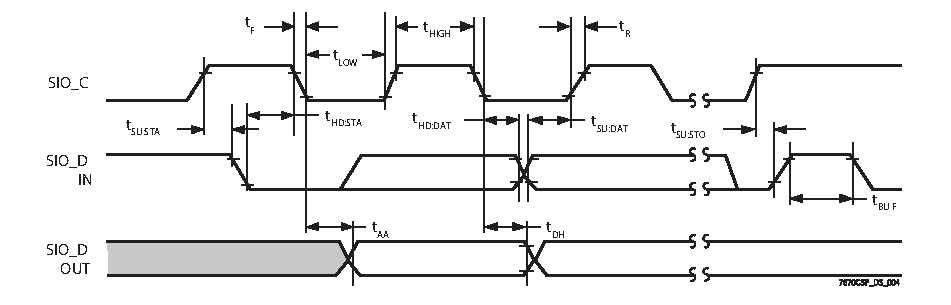
\includegraphics[scale = 1]{OVCam_SCCB.pdf}
				\caption{\it Serial camera control bus waveform}
				\label{fig:SCCB}
			\end{figure}
			

			\item Display data bus\\
			\noindent{The display data bus has the VSYNC signal, HSYNC (or HREF) signal, and D0-D7 for data. The start of the frame signal is defined as the VSYNC signal. Each line of the frame is controlled by the HSYNC signal. \\}
			\newpage
			\begin{figure}[ht!]
				\centering
				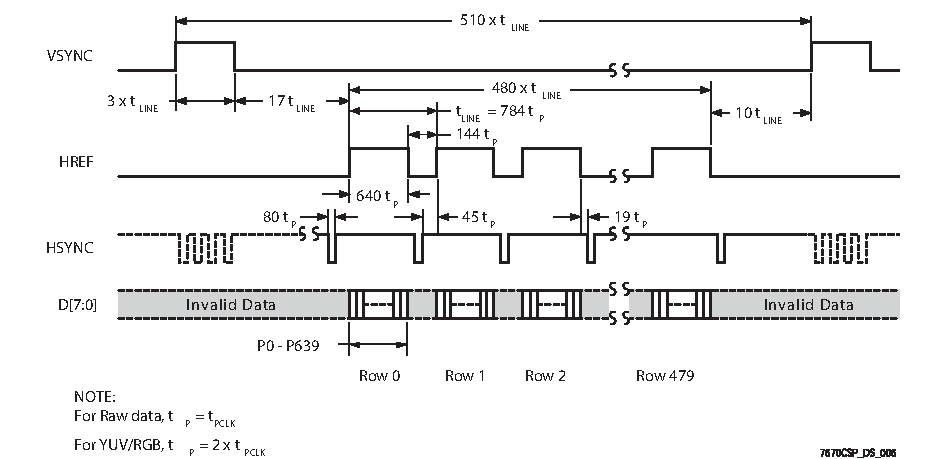
\includegraphics[scale = 1]{Figure/OVCam_dataBus.pdf}
				\caption{\it Display data bus waveform}
				\label{fig:sccbDataBus}
			\end{figure}

			\noindent{Besides, The PCLK is the most important that is synchronous the data output on the data bus. The figure \ref{fig:OneBytes} is showed the waveform of transmission.}
			\begin{figure}[ht!]
				\centering
				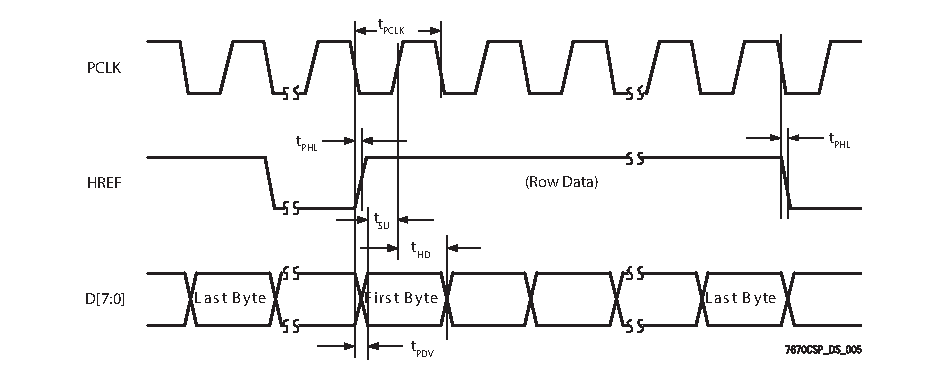
\includegraphics[scale = 1]{Figure/OVCam_OneLine.pdf}
				\caption{\it One bytes data transfer}
				\label{fig:OneBytes}
			\end{figure}
			\newline
		\end{enumerate}

%%%%%%%%%%%%%%%%%%
		\subsection{Memory management}
		\label{subsec:Memory management}
			\subsubsection{MicroController memory organized}
			\label{subsubsec:MicroController Memory}
				The memory intended for the raw data buffer and the jpeg data is too large. If using global memory define at array form, the uninitialized data will be bigger. The space for that memory is too large. Therefore, using dynamic memory is reasonable. \\
				The heap partition is much larger and can be released when don't use it. The raw data buffer needs 38400 bytes of space. The jpeg data is dynamic that can use one KB for simple images and ten KB for complex images. When the required memory is large than the current memory allocated, the processor will automatically reallocate. 
				\begin{figure}[ht!]
					\centering
					\includegraphics[scale = 0.9]{Figure/Memory_Management.pdf}
					\caption{\it Memory management}
					\label{fig:Memory Management}
				\end{figure}
				\subsubsection{RGB565 and YCrCb colour arrangement}
				\label{subsubsec:RGB565}
					For RGB565, each pixel is encoded to 2 bytes. The Red colour use 5 bits, Green is 6 bits and Blue is 5 bits. Sort order as shown in figure \ref{fig:RGB565 ouput waveform} below.	\\
					\begin{figure}[ht!]
						\centering
						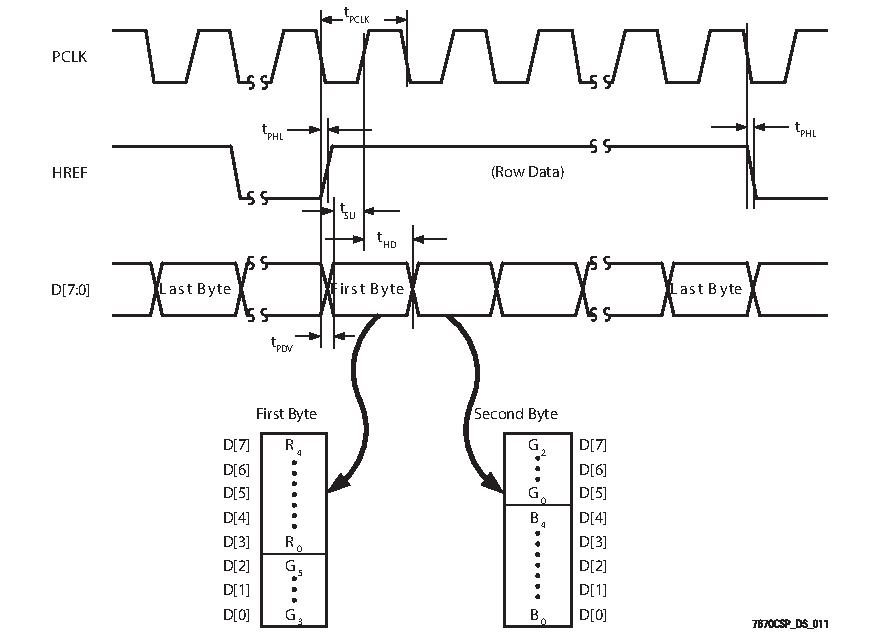
\includegraphics[scale = 0.85]{Figure/Ov_RGB565.pdf}
						\caption{\it RGB565 output waveform}
						\label{fig:RGB565 ouput waveform}
					\end{figure}
					\newline
					For YCbCr, the camera supports the 4:2:2 form. Pixel components are Y (luminance or “luma”), Cb and Cr (chrominance or “chroma” blue and red). Each component is encoded in 8 bits. Luma and chroma are stored together (interleaved) as shown in the figure \ref{fig:YCbCr Colour format in memory} below.	\\
					\begin{figure}[ht!]
						\centering
						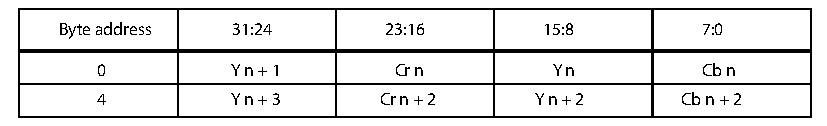
\includegraphics[scale = 1]{Figure/Ov_YCbCr.pdf}
						\caption{\it YCbCr colour format arrange in the memory cell}
						\label{fig:YCbCr Colour format in memory}
					\end{figure}
%%%%%%%%%%%%%%%%%%		
		\subsection{Software achitecture}
		\label{subsec:SoftwareArchitec}
			The software architecture is organized with four layers. \\
			\begin{figure}[ht!]
				\centering
				\includegraphics[scale = 1]{Figure/Software_Architecture.pdf}
				\caption{\it Software architecture}
				\label{fig:Software Architec}
			\end{figure}
			\begin{enumerate}
				\item Driver layer: This layer is used to connect hardware with software. Such as GPIO, DCMI, Uart are controlled at the register layer. 
				\item Hardware abstraction layer: This layer contains STM32HAL and my own HAL {\footnote{Hardware Abstraction Layer}}. My own HAL is built for the OV camera, functions control the camera as color format, exposure, saturation,... 
				\item Middleware layer: At this layer can be RTOS or libjpeg. In this system, the libjpeg is used to convert raw data images to standard jpeg images. 
				\item Application layer: To control the system easier, the software needs to build some functions. Several functions are capture, stop-capture, change camera characterized. Functional tools will be updated in the following section.
			\end{enumerate}
%%%%%%%%%%%%%%%%%%
		\subsection{Software implementation}
		\label{subsec:Software implementation}
			\subsubsection{Capture and transmission timing}
				To optimize in the best way, the stage of one frame process doesn't take place sequentially. It must process continuously. After the system starts to capture the image, the CPU will process line by line the image.  The jpeg image will be transmitted when the processing have already done. \\
				After set up DMA for Uart transmission, the software will get started new capturing. Therefor, the frame rate will be increased. \\
				\begin{figure}[ht!]
					\centering
					\includegraphics[scale = 1]{Figure/Software_Implementation.pdf}
					\caption{\it Capture and transmission timing}
					\label{fig:Captutre and transmission timing}
				\end{figure}
\end{document}